\documentclass[main, 12pt, fleqn]{subfiles}

\begin{document}
\begin{lect} {2019-09-11}

	\begin{lemma}
		$K \subset \R^n$ - компакт, тогда:
		\begin{enumerate}
			\item K - замкн
			\item K - огр
			\item $\forall D \subset K \q D \text{ - замк } \ra D \text{ - комп} $ 
		\end{enumerate}
	\end{lemma}

	\begin{proof} \ \\
	    \begin{figure}[h]
		    \center{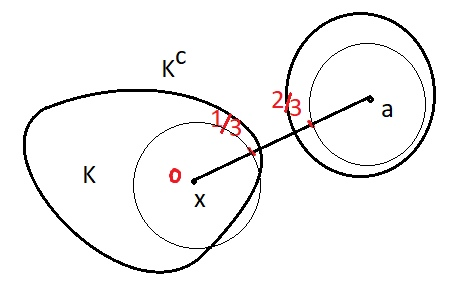
\includegraphics[scale=0.5]{pics/2_1}}
		\end{figure}
	    \[1)\q K^c \ni a\]
		\[\forall x \in K \q d(a, x) > 0\]
		\[r_x = \frac{1}{3} d(x, a)\]
		\[\forall x \in K\]
		\[B(x, r_x) \text{ - откр}\]
		\[K \subset \bigcup_{x \in K} B(x, r_x) \text{ - откр. покр. компакта } K\]
		\[\e x_1, ..., x_N \in K : K \subset \bigcup_{j = 1}^N B(x_j, r_{x_j})\]
		\[a \in \bigcap_{k = 1}^N B(a, r_{x_k}) = B(a, r_{\min}\]
		\[r = \min(r_x, r_{x_N}) > 0\]
		\[\text{ причем } \bigcap_{1}^N B(a, r_{x_k}) \text{ не имеет общих точек}\]
		\[\bigcup_{1}^N B(x_k, r_{x_k})\supset K\]
		\[\e B(a, e_{mn}) \subset K^c \ra K^c \text{ - откр }\ra \text{K - замкн} \]

		\[\text{2) комп - }K \subset \bigcup_{k = 1}^\infty B(0, k) \text{ - откр. покр} \]
		\[\Ra \e k_1, ..., k_n\]
		\[K \subset \bigcup_{j = 1}^N B(0, k_j) = B(0, \max_{1 \leq j \leq N}(k_j)) \Ra K \text{ - огр} \]
		\[\text{3) замкн - }D \subset K \text{ - комп}\]
		Пусть откр. покр
		\[D \subset \bigcup_{\alpha \in A} U_\alpha \]
		\[U^* = D^c \text{ - откр - добавим к покр. K} \{U_\alpha\}_{\alpha \in A}\]
		\[\Ra \text{ выд. конечн. подпокрытие } K \q \{U_{\alpha_j}\}_{j = 1}^N \cup \{U^*\} \]
		\[D \subset \bigcup_{j = 1}^N U_\alpha\]
	\end{proof}
	\begin{theorem}[След. усл. равносильны]
		\begin{enumerate}
			\item K - компакт.
			\item K - замк. и огр.
			\item $\forall \{x_m\}_{m = 1}^\infty \ x_m \in K$
				\[\e \text{ подпосл } x_{m_k} \to x \in K\]
		\end{enumerate}
	\end{theorem}
	\begin{proof}
		$(1 \Ra 2)$ было\\
		$(2 \Ra 1)$
		\[\text{т.к. } K \text{ - огр} \Ra \e I = \prod_{j = 1}^n [a_j, b_j]\]
		\[\text{замкн - }K \subset I \text{ - комп}\]
		$\Ra$ (лемма) K - комп\\
		$(2 \Ra 3)$
		\[x_m \in K \text{ - замк и огр}\]
		\[\Ra \e x_{m_k} \text{ - сх (пр. выб. Б-В)}\]
		\[x_{m_k} \to x \text{ предпол } x \not \in K\]
		\[x \in K^c \text{ - откр } \Ra \e B_x \subset K^c\]
		\[\text{Но } K \ni d(x_{m_k}, x) \to 0 \text{ противореч } x \in K \]
		$(3 \ra 2)$
		\[\text{а) предп.} K \text{ не явл. огр.} \]
		\[\forall n \in \N \q \e x_n \in K: d(0, x_n) > n\]
		\[\{x_n\} \text{ не огр} \Ra \text{ не сх.}\]
		\[\Ra K \text{ - огр}\]
		\[\text{б) предп., что } K \text{ - не явл. замкн}\]
		\[K^c \text{ - не откр }\]
		\[\e a \in K^c : \forall \delta > 0 \  B(a, \delta) \cap K \neq \varnothing\]
		\[\e x_n \in B(a, \frac{1}{n}) \cap K\]
		\[x_n \in K\]
		\[0 \leq d(x_n, a) < \frac{1}{n} \to 0 \q x_n \to a; \ x_{n_k} \to x \in K\]
	\end{proof}
	
	\begin{upr}
	    \[K_1 \supset K_2 \supset ...\]
		\[\text{д-ть } \bigcap_{j \in \N} K_j \neq \varnothing\]
	\end{upr}
	
	\section{Отображения в $\R^n$}
	\begin{Definition}
		\[E \subset \R^n,\q f: E \to \R^m \text{ - отобр-е (вект. ф-я)}\]
		\[(m = 1 \text{ - ф-я})\]
		\[f(x) = (f_1(x), ..., f_m(x))\]
		\[x= (x_1, ..., x_n) \q f_j: E \to \R \text{ коорд. функ-ия}\]
	\end{Definition}
	\begin{Definition}
	    \[a \in \R^n\]
		\[a \text{ - пред. т. E, если }\]
		\[\forall \delta > 0 \q U()(a, \delta) \cap E \neq \varnothing\]
	\end{Definition}
	\begin{definition}
		\[f: E \to \R^m, a \text{ - пред. т E}\]
		\[\lim_{x \to a} f(x) = L \text{, если}\]
		\[\text{(Коши }) \forall \E > 0 \q \e \delta > 0 : \forall x \in E\]
		\[0 < d(x, a) < \delta \ra d(f(x), L) < \E\]
		\[\text{(Гейне) } \forall \{x_k\}_{k = 1}^\infty \q x_k \in E \setminus \{a\} x_k \to_{k \to \infty} a  \ra F(x_k) \to_{k \to \infty} L \]
	\end{definition}
	\begin{upr}
	    Эквивалентность определений
	\end{upr}
	\begin{upr}
	    Сходимость $\lra$ покоординатная сходимость
	\end{upr}
	
	\begin{example}
		\[f(x, y) = \left\{ \begin{align}
				&\frac{xy}{x^2 + y^2}, & (x,y) \neq (0, 0)\\
				&0, & (x,y) = (0, 0)
		\end{align}\]
		Повторные пределы
		\[\lim_{x \to 0} \lim_{y \to 0} f(x, y) = 0\]
		\[\lim_{y \to 0} \lim_{x \to 0} f(x, y) = 0 \]
		\[f(\delta, \delta) = \frac{1}{2} \underset{\delta \to 0}{\to}\frac{1}{2}\]
		\[f(\delta, -\delta) = -\frac{1}{2}\]
		\[\text{т.е } \lim_{(x, y) \to (0,0)} f(x, y) \text{ не сущ.} \]
	\end{example}

	\begin{Theorem}[предел композиции]
			\[E \subset \R^n, \q F \subset \R^m \q\q \R^n \ni a \text{ - пред т. E} \ F \ni b \text{ - пред. т. F}\]
			\[f: E \to F; \q g: F \to \R^l\]
			\[\lim_{x \to a} f(x) = b; \q \lim_{x \to b} g(x) = g(b) \]
			\begin{figure}[h]
    		    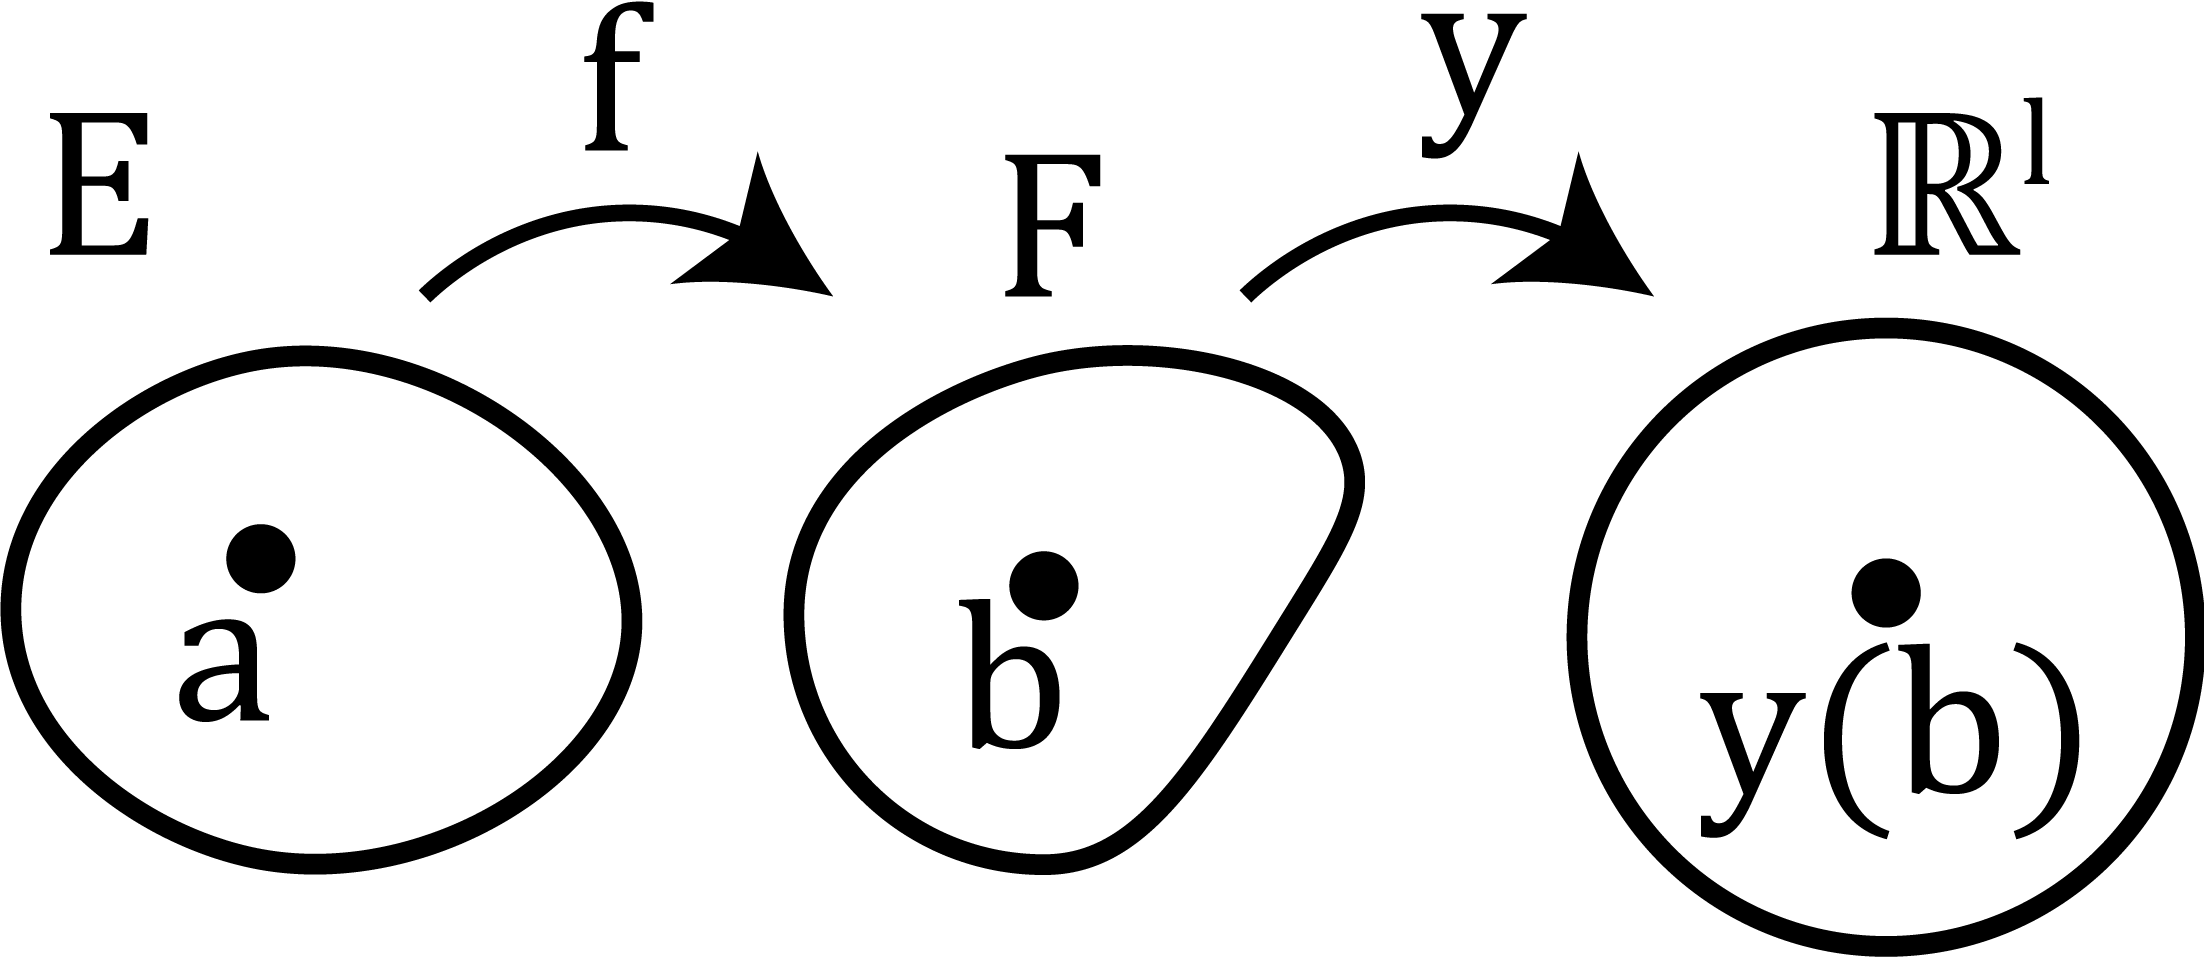
\includegraphics[scale=0.5]{pics/2_2}
    		    \centering
    		\end{figure}
			\[\text{ Тогда } \lim_{x \to a} g \circ f = g(b) \]
	\end{Theorem}
	\begin{Theorem}[Крит. Коши]
			\[a \text{ - пред т. } E\]
			\[f(x) \text{ имеет предел в т.} a\]
			\[ \rla \forall \E > 0 \e \delta > 0 : 
			\forall x, y \in \doted{U}(a, \delta) \cap E \ra d(f(x), f(y)) < \E\]
	\end{Theorem}
	
	\addcontentsline{toc}{subsection}{Непрерывные отображения}
	\begin{Definition} [непрерывные отображения]
			\[a \in E \q\q f: E \to \R^m\]
			Если $a$ - изол $\ra f$ - непр в $a$,\\
			если $a$ - пред, то $f \text{ - непр в т. } a \rla $\\
			\[\rla \lim_{x \to a}f(x) = f(a) \]
			\[f \text{ - непр в т.} a \rla f_j \text{ - непр. в т } a \ \forall 1 \leq j \leq m\]
			\[f \text{ - непр в т. } a; g \text{ - непр в } f(a) \rla g \circ f \text{ - непр в т } a\]
			\[\text{непр сохр. при +, умн. на число}\]
			\[f \text{ - непр на } E \rla \text{ непр } \forall a \in E\]
	\end{Definition}

	\begin{Theorem}[эквивалентность определений непрерывности]
			\[f: E \to \R^m\]
			\[f \text{ - непр на } E \rla \forall G \subset \R^m \q G \text{ - откр } \ra 
			f^{-1}(G) \text{ - откр в } E\]
	\end{Theorem}

	\begin{Proof}
		\[G \text{ - откр.}\]
		\[f^{-1}(G) \text{ - откр ?}\]
		\begin{figure}[h]
		    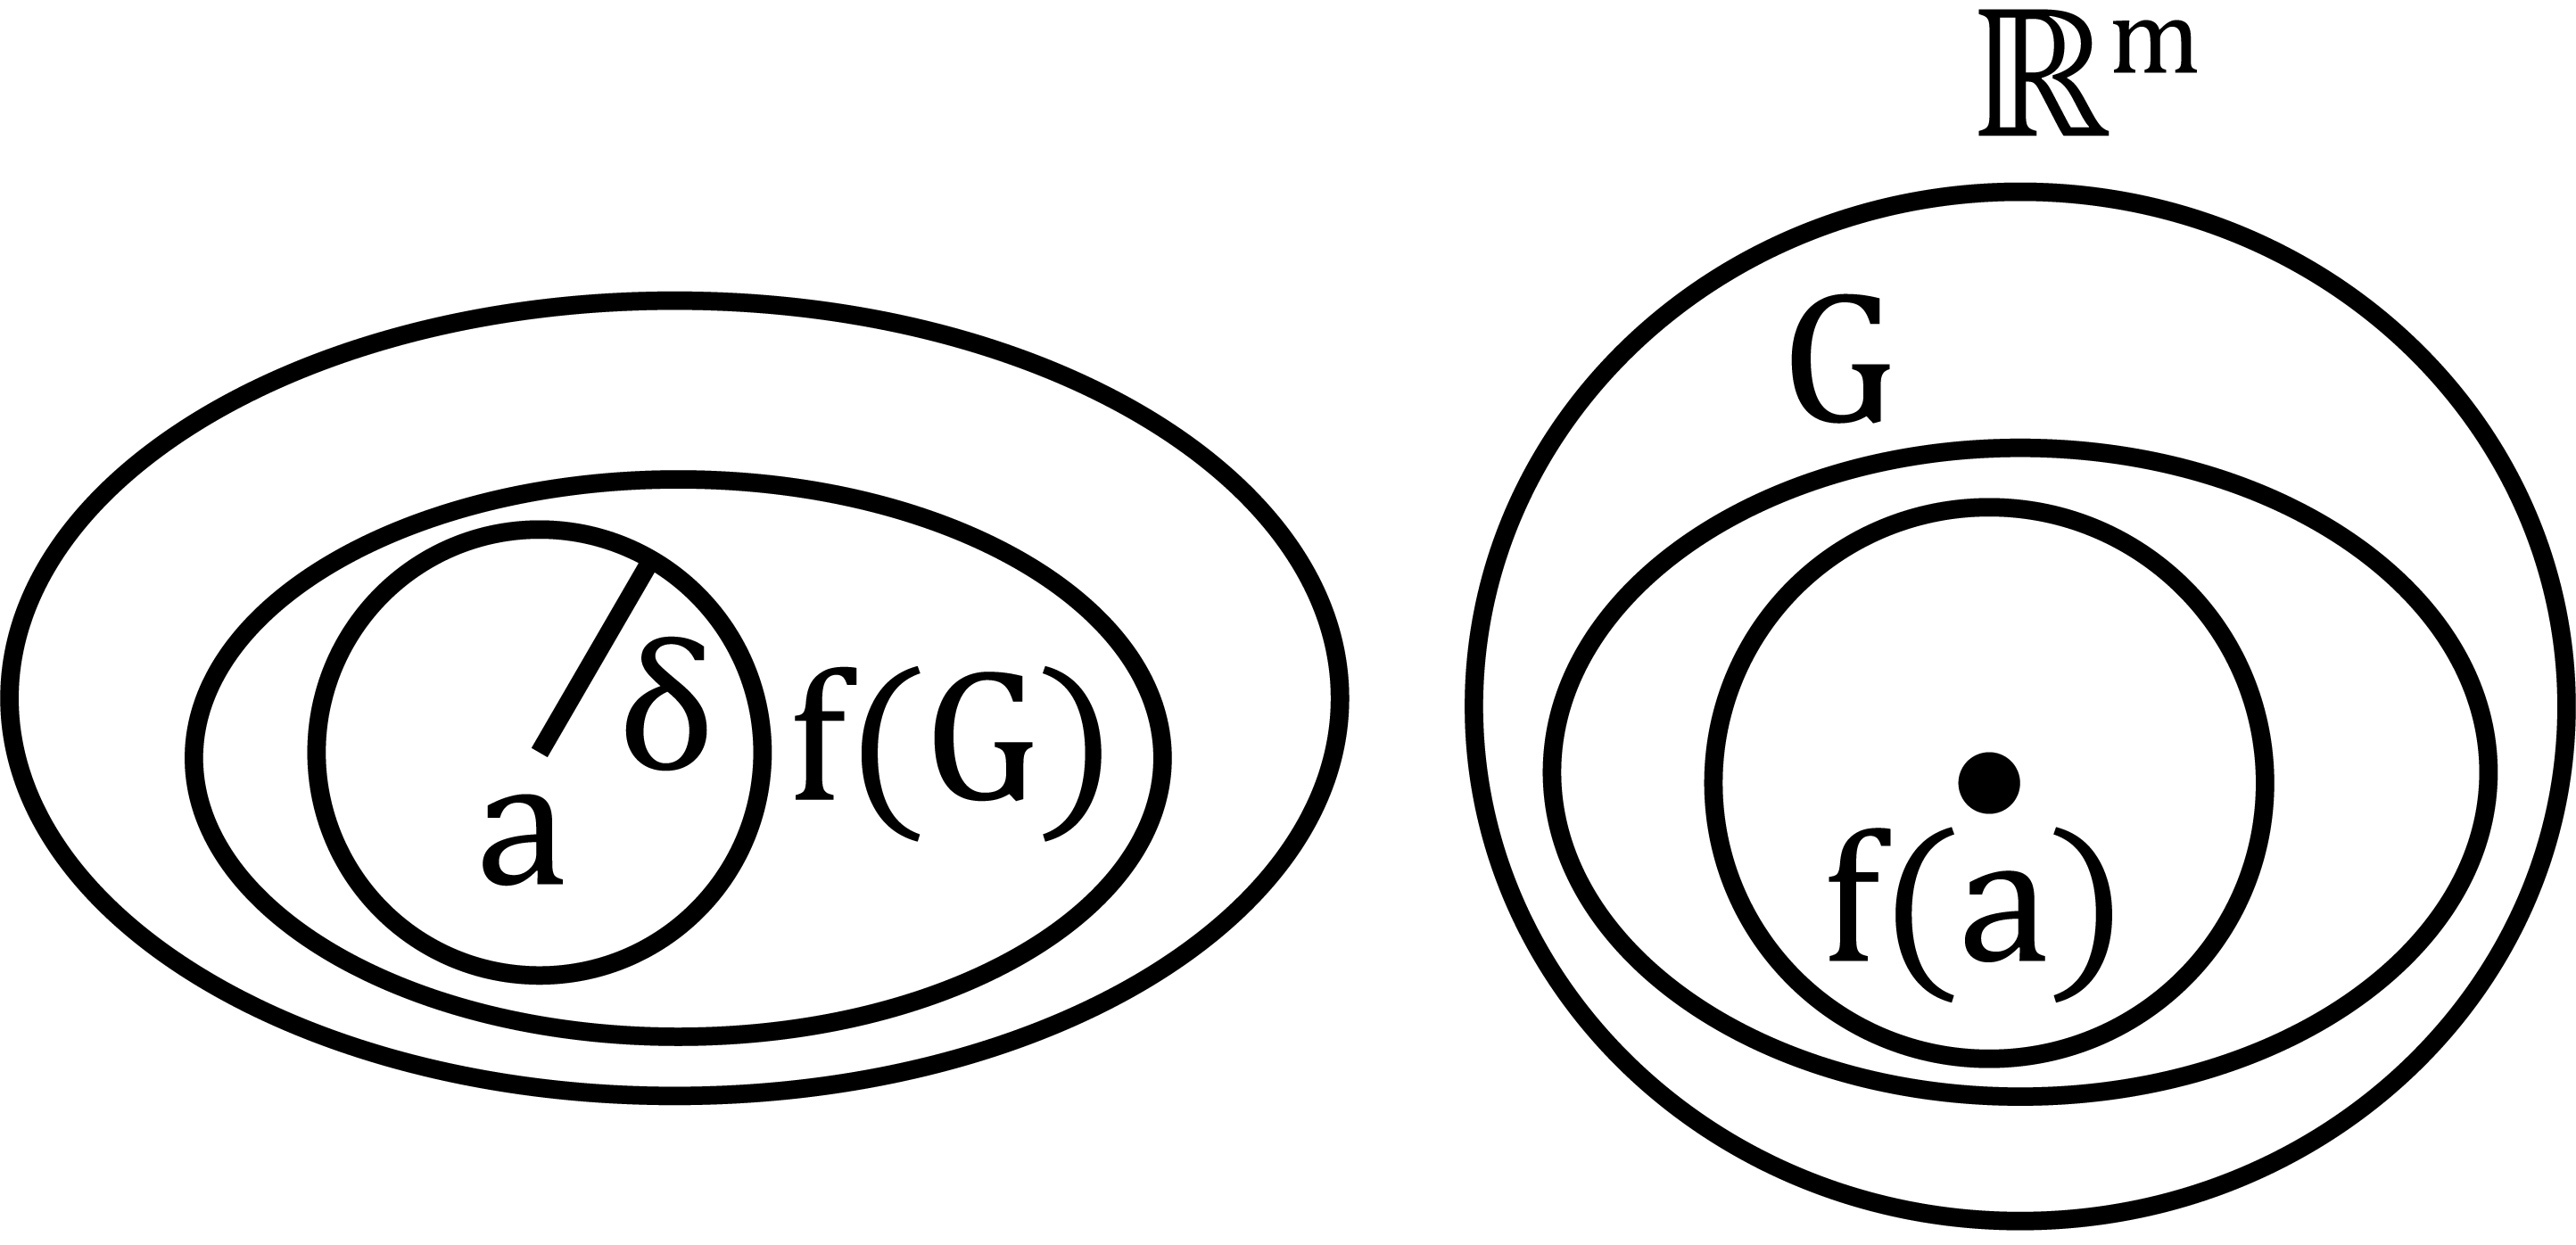
\includegraphics[scale=0.5]{pics/2_3}
		    \centering
		\end{figure}
		\[a \in f^{-1}(G)\]
		\[f(a) \in G \text{ - откр } \ra \e U(f(a), \E) \subset G\]
		рисунок
		\[\text{т.к } f \text{ непр в т. } a \]
		\[\e \delta : d(a, x) < \delta \ra d(f(a), f(x)) < \E\]
		\[f(B(a, \delta)) \subset B(f(a), \E) \subset G\]
		\[\ra B(a, \delta) \subset f^{-1}(G)\]
		\[\la a \in E \ra ? f \text{ - непр в т. a} \text{ (рисунок)}\]
		\begin{figure}[h]
		    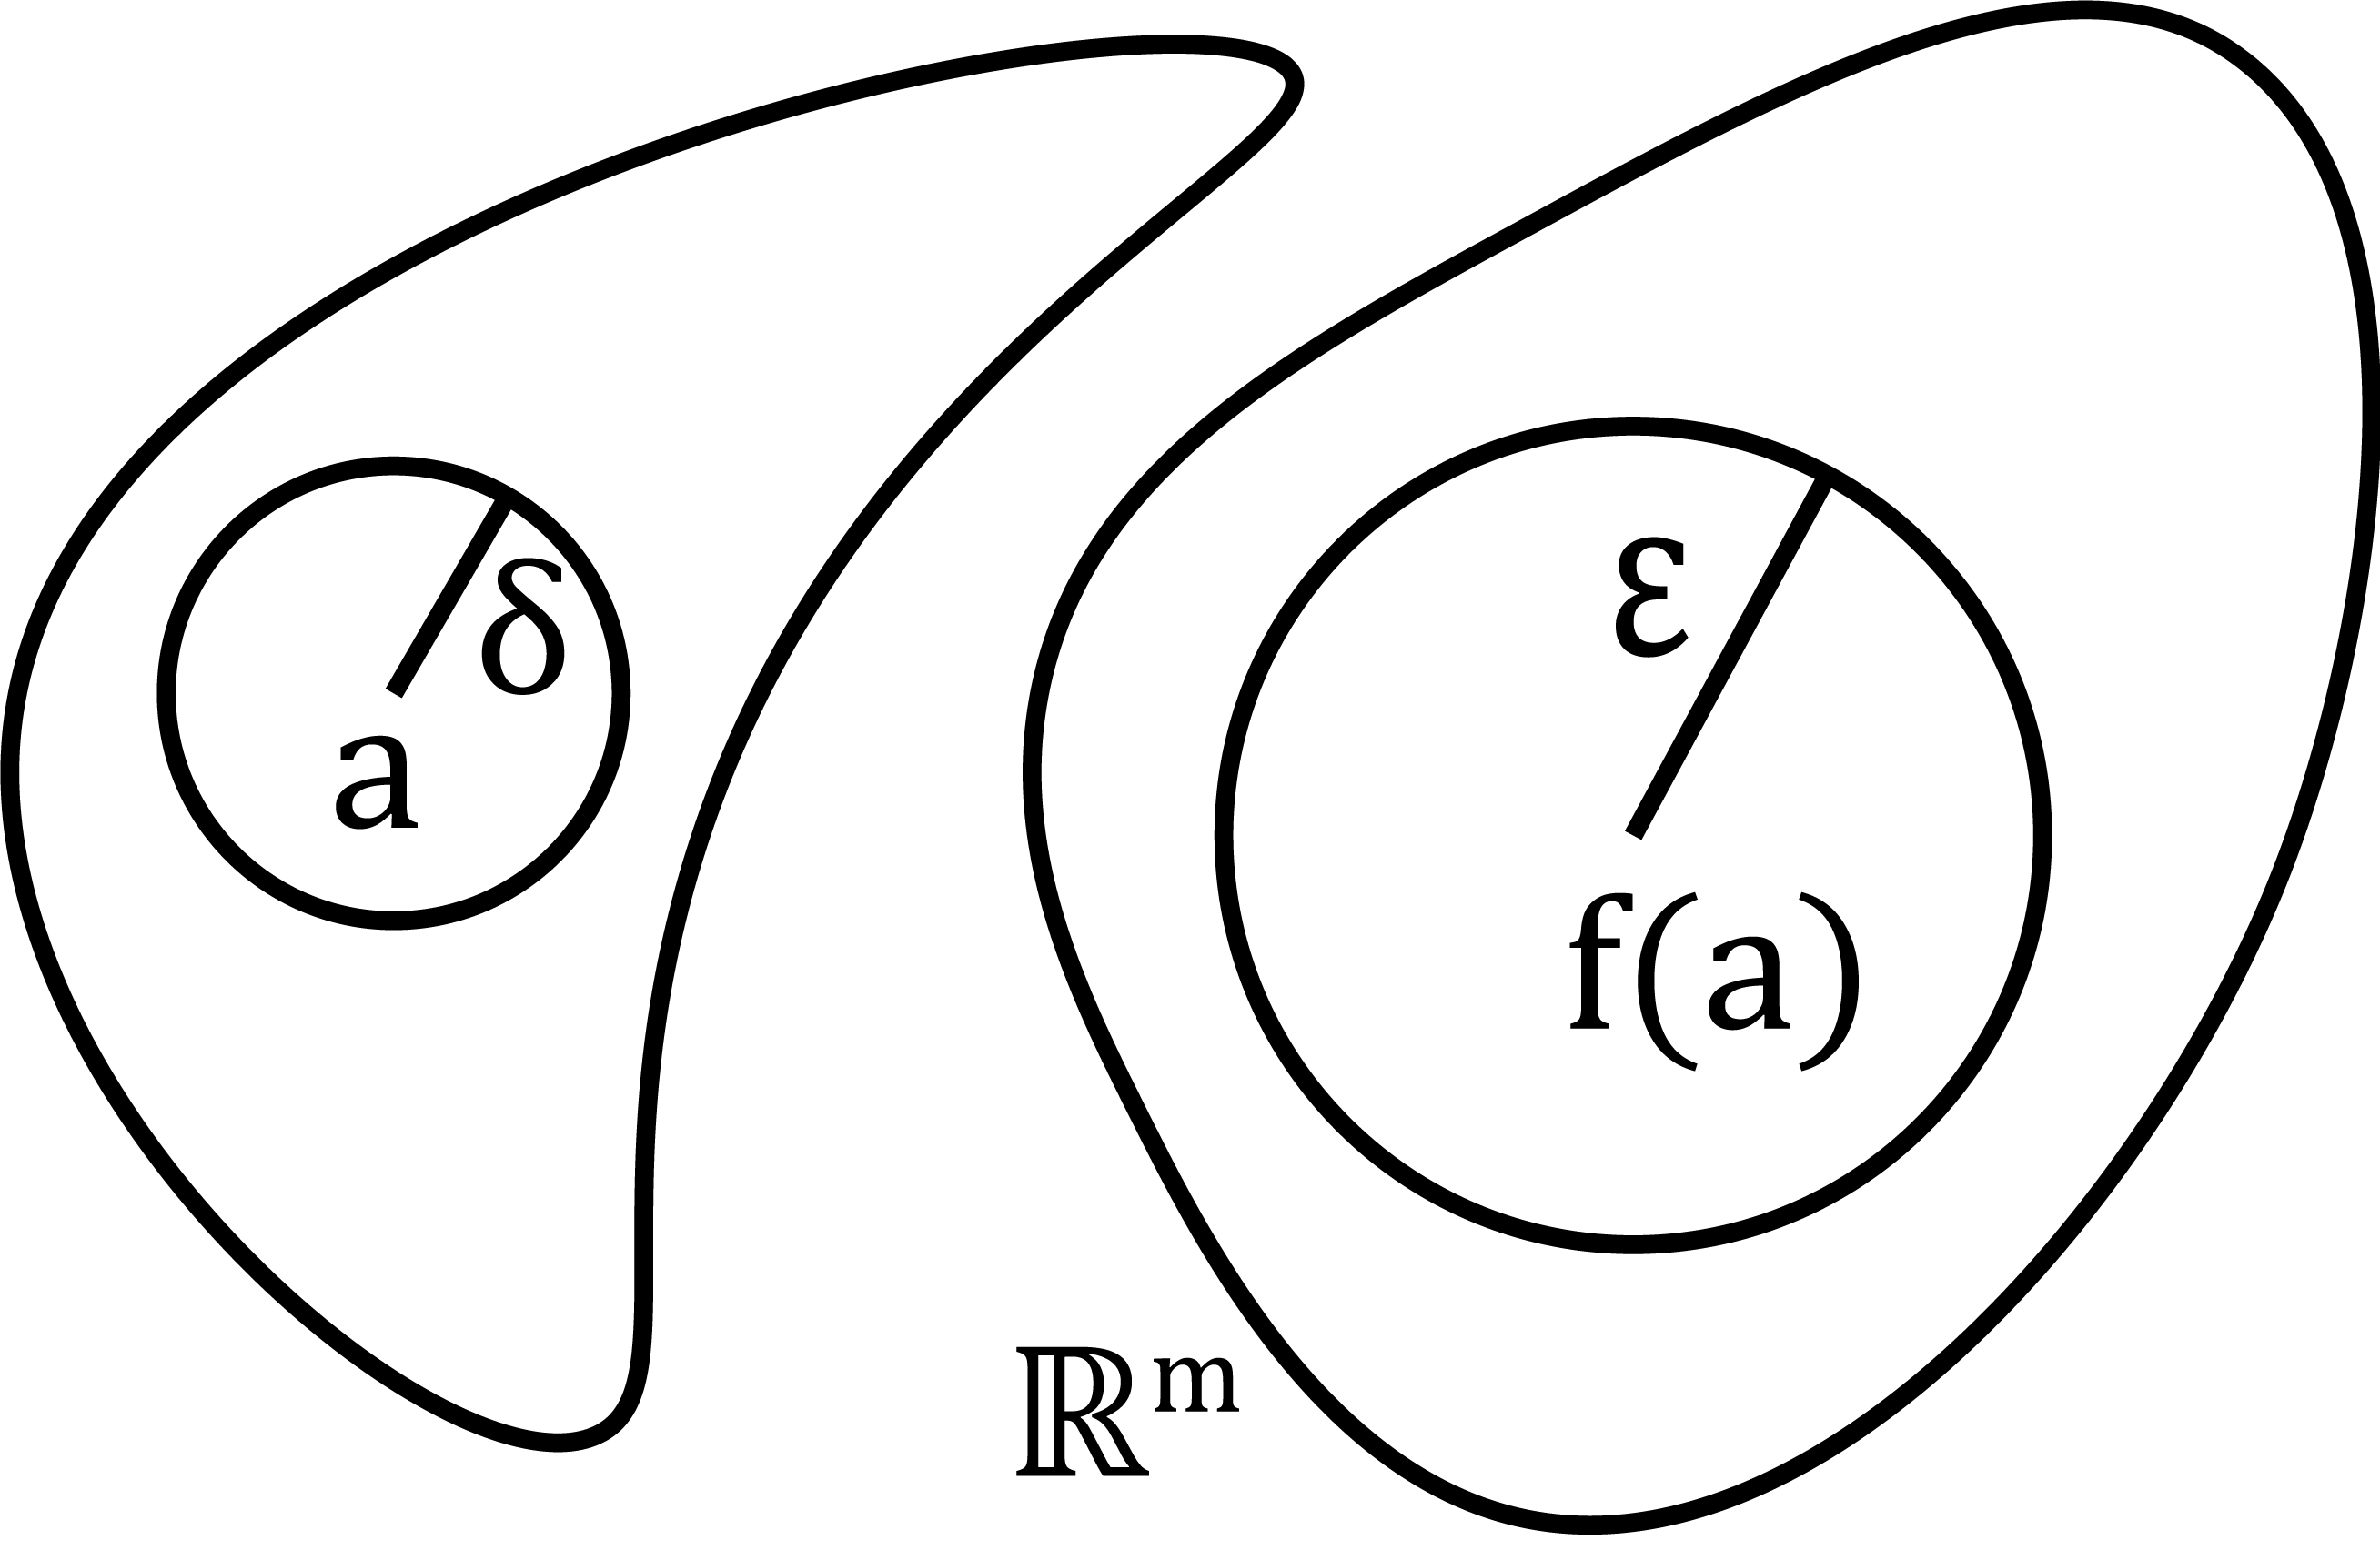
\includegraphics[scale=0.5]{pics/2_4}
		    \centering
		\end{figure}
		
		\[\forall \E > 0 B(f(a), \E) \text{ - откр в } \R^m\]
		\[\ra f^{-1}(B(f(a), \E) \text{ - откр.} \ra \e \delta : B(a, \delta) \subset f^{-1}
		(B(f(a), \E)) \ra f \text{ - непр. в т } a\]
		
	\end{Proof}
    
    \addcontentsline{toc}{subsection}{Локальные свойства непрерывности}
	\begin{theorem}[локальные свойства непр. функций]
	    (дописать)
		\begin{enumerate}
			\item непрерывна в т. a $\Ra$ найдетс
			\item f - непр в т. a; g непр в a, $f \circ g$ непр в a. 
			\item f - непр в т. а, g - непр в f(a) $\Ra$
		\end{enumerate}
	\end{theorem}
\end{lect}
\end{document}